\documentclass{exam}
\usepackage[utf8]{inputenc}
\usepackage{lmodern}
\usepackage{microtype}

% \usepackage[parfill]{parskip}
\usepackage[dvipsnames]{xcolor}
\usepackage{amsmath}
\usepackage{amsfonts}
\usepackage{amsthm}
\usepackage{siunitx}
\DeclareSIUnit\year{yr}
\DeclareSIUnit\foot{ft}
\DeclareSIUnit\litre{\liter}

\usepackage{skull}

\usepackage{pgfplots}
\usepgfplotslibrary{polar}
\pgfplotsset{compat=1.11}
\usepgfplotslibrary{statistics}
\usepackage{graphicx}
\usepackage{sidecap}
\sidecaptionvpos{figure}{c}
\usepackage{float}
\usepackage{gensymb}
\usepackage{tkz-euclide}
\usetkzobj{all}
\usepackage{commath}
\usepackage{hyperref}
\usepackage{enumitem}
\usepackage{wasysym}
\usepackage{multicol}
\usepackage{mathtools}
\usepackage{tcolorbox}
\usepackage{tabularx}
\usepackage[version=4]{mhchem}
\usepackage{changepage}
\usepackage{listings}
\lstset{basicstyle=\ttfamily\linespread{0.8}\small}

\renewcommand*{\thefootnote}{\fnsymbol{footnote}}

\newtheorem*{thm}{Theorem}
\newtheorem*{iden}{Identity}
\newtheorem*{lemma}{Lemma}
\newtheorem{obs}{Observation}
\theoremstyle{definition}
\newtheorem*{defn}{Definition}
\newtheorem*{ex}{Example}
\newtheorem{con}{Construction}
\newtheorem*{alg}{Algorithm}

\newtheoremstyle{break}
  {\topsep}{\topsep}%
  {\itshape}{}%
  {\bfseries}{}%
  {\newline}{}%
\theoremstyle{break}
\newtheorem*{bthm}{Theorem}

% russian integral
\usepackage{scalerel}
\DeclareMathOperator*{\rint}{\scalerel*{\rotatebox{17}{$\!\int\!$}}{\int}}

% \DeclareMathOperator*{\rint}{\int}

\pgfplotsset{vasymptote/.style={
    before end axis/.append code={
        \draw[densely dashed] ({rel axis cs:0,0} -| {axis cs:#1,0})
        -- ({rel axis cs:0,1} -| {axis cs:#1,0});
    }
}}

% \pointsinrightmargin
\boxedpoints
\pointname{}

\newcommand{\questioA}{\question[\texttt{\textbf{\color{Cerulean} A}}]}
\newcommand{\questioM}{\question[\texttt{\textbf{\color{PineGreen} M}}]}
\newcommand{\questioE}{\question[\texttt{\textbf{\color{WildStrawberry} E}}]}
\newcommand{\questioS}{\question[\texttt{\textbf{\color{Goldenrod} S}}]}
\newcommand{\questioO}{\question[\texttt{\textbf{\color{BurntOrange} O}}]}

\newcommand{\parA}{\part[\texttt{\textbf{\color{Cerulean} A}}]}
\newcommand{\parM}{\part[\texttt{\textbf{\color{PineGreen} M}}]}
\newcommand{\parE}{\part[\texttt{\textbf{\color{WildStrawberry} E}}]}
\newcommand{\parS}{\part[\texttt{\textbf{\color{Goldenrod} S}}]}
\newcommand{\parO}{\part[\texttt{\textbf{\color{BurntOrange} O}}]}

\newcommand{\subparA}{\subpart[\texttt{\textbf{\color{Cerulean} A}}]}
\newcommand{\subparM}{\subpart[\texttt{\textbf{\color{PineGreen} M}}]}
\newcommand{\subparE}{\subpart[\texttt{\textbf{\color{WildStrawberry} E}}]}
\newcommand{\subparS}{\subpart[\texttt{\textbf{\color{Goldenrod} S}}]}
\newcommand{\subparO}{\subpart[\texttt{\textbf{\color{BurntOrange} O}}]}

\newcommand{\mainHeader}[2]{\section*{NCEA Level 2 Mathematics\\#1. #2}}
\newcommand{\mainHeaderHw}[2]{\section*{NCEA Level 2 Mathematics (Homework)\\#1. #2}}
\newcommand{\seealso}[1]{\begin{center}\emph{See also #1.}\end{center}}
\newcommand{\drills}[1]{\begin{center}\emph{Drill problems: #1.}\end{center}}
\newcommand{\basedon}[1]{\begin{center}\emph{Notes largely based on #1.}\end{center}}

\begin{document}

\mainHeaderDiff{10}{Inverse Functions}
We need to take a quick pitstop this week to deal with one more differentiation rule before we can start looking at a few more applications
next week and then some interesting functions in higher dimensions later on.

\begin{defn}
  A function is called \textbf{one-to-one} (or \textbf{injective}) if $ f(x) = f(y) $ implies that $ x = y $ (i.e. two different inputs can never
  give the same output/the function passes the horizontal-line test).

  Let $ f $ be a function that is one-to-one. Then the \textbf{inverse} of $ f $ is the (unique) function $ f^{-1} $ such that
  \begin{displaymath}
    f(x) = y \iff f^{-1}(y) = x.
  \end{displaymath}
  In other words, $ f(f^{-1}(y)) = y $ and $ f^{-1}(f(x)) = x $.
\end{defn}

\begin{ex}
  Here are some functions with their inverses:
  \begin{center}
  \def\arraystretch{1.5}
  \begin{tabularx}{0.9\linewidth}{|c|c|X|}\hline
    \textbf{Function} & \textbf{Inverse} & \textbf{Notes}\\\hline
    $ e^x $ & $ \ln x $ & Note that $ \ln x $ is defined only when $ x > 0 $ since $ e^x > 0 $ for all real $ x $.\\
    $ \sin x $ & $ \sin^{-1} x $ & Note that $ \sin^{-1} x $ is only defined when $ -\pi < x \leq \pi $ since otherwise $ \sin x $ is not one-to-one.\\
    $ \cos x $ & $ \cos^{-1} x $ & Note that $ \cos^{-1} x $ is only defined when $ -\pi < x \leq \pi $ since otherwise $ \cos x $ is not one-to-one.\\
    $ \tan x $ & $ \tan^{-1} x $ & Note that $ \tan^{-1} x $ is defined for all $ x $ (why?), and so $ \tan^{-1} x \neq \frac{\sin^{-1} x}{\cos^{-1} x} $.\\
    $ x^2 $ & $ \sqrt{x} $ & When $ x $ is positive.\\\hline
  \end{tabularx}
  \end{center}
\end{ex}
The graph of the inverse of a function is the reflection of the graph of the original function around the line $ x = y $ (essentially, we swap
the $ x $ and $ y $ axes).

\begin{thm}
  In general, if $ f $ is a function passing through $ (x,y) $, and $ f^{-1} $ is the inverse of $ f $, then
  \begin{displaymath}
    (f^{-1})'(y) = \frac{1}{f'(f^{-1}(y))} = \frac{1}{f'(x)}.
  \end{displaymath}
  Mnemonically, we can write this as
  \begin{displaymath}
    \od{x}{y} = \frac{1}{\od{y}{x}}.
  \end{displaymath}
\end{thm}
\begin{proof}
  We have that $ f(f^{-1}(y)) = y $. Taking the derivative of both sides, $ f'(f^{-1}(y)) \cdot (f^{-1})'(y) = 1 $
  and therefore $ (f^{-1})'(y) = \frac{1}{f'(f^{-1}(y))} $.
\end{proof}

This proof is not hard, but it is sometimes difficult to work out which $ x$'s and $ y$'s go where. We'll do a couple of examples now; the
first one is one that we can already do, and so this gives us the advantage of knowing what the result should look like before we get there.

\begin{ex}
  Suppose $ f $ is defined by $ y = f(x) = x^2 $. Then $ f^{-1}(y) = \sqrt{y} $. We evaluate it in three ways.
  \begin{enumerate}
    \item Power law: $ f^{-1}(y) = y^{\frac{1}{2}} $ so $ (f^{-1})(y) = \frac{1}{2} y^{-\frac{1}{2}} = \frac{1}{2\sqrt{y}} $.
    \item Rigourous derivative of inverse: We have that $ (f^{-1})'(y) = \frac{1}{f'(f^{-1}(y))} $, so $ (\sqrt{y})' = \frac{1}{2\sqrt{y}} $ (since $ f'(x) = 2x $).
    \item Mnemonic derivative of inverse:  We wish to find $ \od{x}{y} $. Now $ \od{y}{x} = 2x $ and so (by the mnemonic)
          \begin{displaymath}
            (f^{-1})'(y) = \od{x}{y} = \frac{1}{\od{y}{x}} = \frac{1}{2x} = \frac{1}{2\sqrt{y}}.
          \end{displaymath}
  \end{enumerate}
\end{ex}

\begin{ex}
  In order to illustrate the general process of finding the derivatives of inverse functions without symbol-pushing using the theorem above, let us
  now find the derivative of $ y = \sin^{-1} x $.
  \begin{align*}
    y &= \sin^{-1} x\\
    \sin y &= x\\
    \dod{y}{x} \cos y &= 1\\
    \dod{y}{x} &= \frac{1}{\cos y} = \frac{1}{\cos \sin^{-1} x} = \frac{1}{\sqrt{1 - x^2}}.
  \end{align*}
  The identity $ \cos\sin^{-1} x = \sqrt{1 - x^2} $ comes from the following triangle:
  \begin{center}
    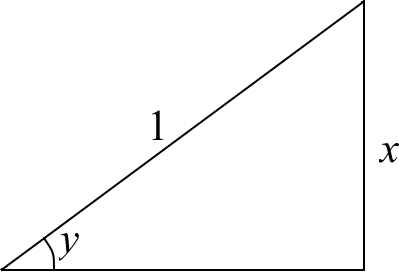
\includegraphics[width=0.2\textwidth]{antitriangle}
  \end{center}
\end{ex}

By the same kind of calculation, we obtain the following table which gives the derivatives of inverses of the three primary trigonometric
functions and their reciprocals.
\begin{center}
  \def\arraystretch{1.8}
  \begin{tabular}{|c|c|c|c|}\hline
    \textbf{Function} & \textbf{Derivative} &
    \textbf{Function} & \textbf{Derivative}\\\hline
    $ \sin^{-1} x $ & $ \dfrac{1}{\sqrt{1 - x^2}} $ &
    $ \csc^{-1} x $ & $ -\dfrac{1}{x\sqrt{x^2 - 1}} $ \\\hline
    $ \cos^{-1} x $ & $ -\dfrac{1}{\sqrt{1 - x^2}} $ &
    $ \sec^{-1} x $ & $ \dfrac{1}{x\sqrt{x^2 - 1}} $\\\hline
    $ \tan^{-1} x $ & $ \dfrac{1}{1 + x^2} $ &
    $ \cot^{-1} x $ & $ -\dfrac{1}{x^2 + 1}$\\\hline
  \end{tabular}
\end{center}

\subsection*{Questions}
\begin{questions}
  \questioM Prove or disprove the following statements:
    \begin{parts}
      \part The function $ f : x \mapsto x^2 + x + 1 $ is one-to-one (where $ x $ is real).
      \part The function $ g : x \mapsto 2^x $ is one-to-one (where $ x $ is a positive real).
    \end{parts}
  \questioM Determine whether the following functions have inverses on the given interval:
    \begin{parts}
      \part $ x \mapsto x^3 $ (on $ \mathbb{R} $)
      \part $ y \mapsto y^4 $ (on $ \mathbb{R} $)
      \part $ y \mapsto y^4 $ (for $ y \geq 0 $)
      \part $ y \mapsto y^4 $ (for $ y > 0 $)
      \part $ \theta \mapsto \cos^{-1} \theta $ (on $ \mathbb{R} $)
      \part $ \theta \mapsto \cos^{-1} \theta $ (for $ -1 \leq \theta \leq 1 $)
    \end{parts}
  \questioA True or false:
    \begin{parts}
      \part $ \cos^{-1} x = \frac{1}{\cos x} $
      \part If $ x > 0 $ then $ (\ln x)^6 = 6\ln x $
      \part $ \tan^{-1} (-1) = \frac{3\pi}{4} $ (think about which arm of $ \tan x $ we're talking about)
      \part The inverse of $ f(x) = e^{3x} $ is $ f^{-1}(x) = \frac{1}{3} \ln x $.
    \end{parts}
  \questioA Find the derivative of $ f(x) = \ln(e^x) $ in two different ways.
  \questioA Find $ y' $ if:
    \begin{parts}
      \part $ y = \sin^{-1} 2x $
      \part $ x = \sin^2 y $
      \part $ y = x + \tan^{-1} y $
      \part $ y = \ln \sin x - \frac{1}{2} \sin^2 x $
      \part $ y = 24\arctan x + \arcsin \sqrt{x} $
      \part $ y = \sqrt{\sec^{-1} 2x} $
    \end{parts}
  \questioE Find the local extrema, areas of concavity, and inflection points of the following functions; hence sketch their graphs.
    \begin{parts}
      \part $ y = e^x \sin x $ for $ -\pi < x < \pi $
      \part $ y = x + \ln(x^2 + 1) $
      \part $ y = \sin^{-1} (1/x) $
    \end{parts}
  \questioE Justify intuitively, without invoking the happy coincidence that our notation for derivatives looks like a fraction, the
            statement that $ \od{y}{x} = \left(\od{x}{y}\right)^{-1} $.
  \questioE If $ f'(x) = \tan^{-1} x $, find $ (f^{-1})'(x) $.
  \questioE Using the definition of $ \ln $ as the inverse of $ \exp : x \mapsto e^x $, show that $ \od{}{x} \ln x = \frac{1}{x} $. \textit{Note
            that the usual definition of $ \ln $ goes in the reverse of this; we will go in that direction in a few weeks.}
  \questioS Prove the formulae for the derivatives of $ \cos^{-1} $ and $ \tan^{-1} $, using a similar method to that for $ \sin^{-1} x $.
  \questioS Scholarship 2012: Consider the equation $ x^n = \tan(ny) $, where $ n $ is a constant. Find an expression
            for $ \od{y}{x} $ in terms of $ x $.
  \questioS Scholarship 2017: The functions $ \sinh $ and $ \cosh $ are defined as follows.
            \begin{align*}
              \sinh x &= \frac{1}{2}\left(e^x - e^{-x}\right),\\
              \cosh x &= \frac{1}{2}\left(e^x + e^{-x}\right).
            \end{align*}
            The inverse function of $ \sinh $ is denoted by $ \sinh^{-1} $. By implicit differentiation, or
            otherwise, show that
            \begin{displaymath}
              \od{}{x} \sinh^{-1} x = \frac{1}{\sqrt{x^2 + 1}}.
            \end{displaymath}
\end{questions}
\end{document}
